\documentclass[a4paper,10pt]{article}
%\documentclass[a4paper,10pt]{scrartcl}

\usepackage{xltxtra}
\usepackage{fullpage}

\setromanfont[Mapping=tex-text]{Linux Libertine O}
% \setsansfont[Mapping=tex-text]{DejaVu Sans}
% \setmonofont[Mapping=tex-text]{DejaVu Sans Mono}

\title{Grid User Guide}
\author{Amy de Buitléir}

\begin{document}
\maketitle

\section{Square tiles}

\texttt{rectSquareGrid r c} returns a rectangular grid with \texttt{r} rows and \texttt{c} columns, using square tiles.
The indexing scheme is illustrated in Figure \ref{fig:rectSquareGrid}.

\begin{figure}[ht]
 \label{fig:rectSquareGrid}
 \centering
 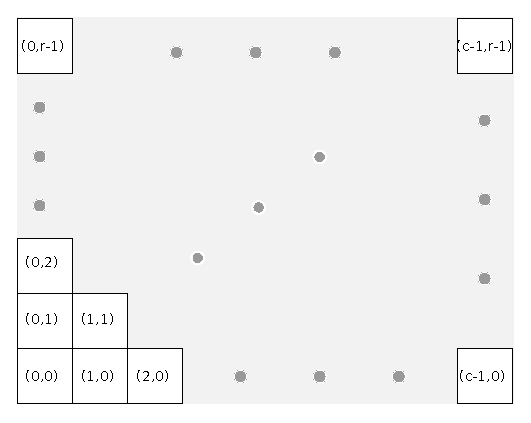
\includegraphics{./images/rectSquareGrid.eps}
 \caption{Grid generated by \texttt{rectSquareGrid}}
\end{figure}


\texttt{torSquareGrid r c} returns a toroidal grid with \texttt{r} rows and \texttt{c} columns, using square tiles.
The indexing scheme is illustrated in Figure \ref{fig:torSquareGrid}.

\begin{figure}[ht]
 \label{fig:torSquareGrid}
 \centering
 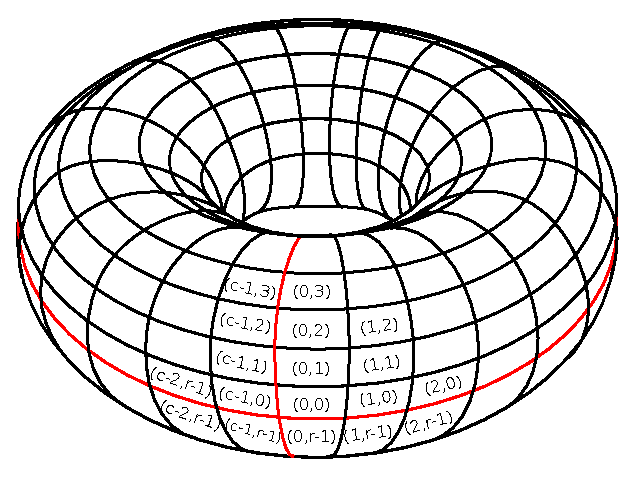
\includegraphics{./images/torSquareGrid.eps}
 \caption{Grid generated by \texttt{torSquareGrid}}
\end{figure}


\section{Triangular tiles}

\texttt{triTriGrid s} returns a triangular grid with sides of length \texttt{s}, using triangular tiles.
The indexing scheme is illustrated in Figure \ref{fig:triTriGrid}.

\begin{figure}[ht]
 \label{fig:triTriGrid}
 \centering
 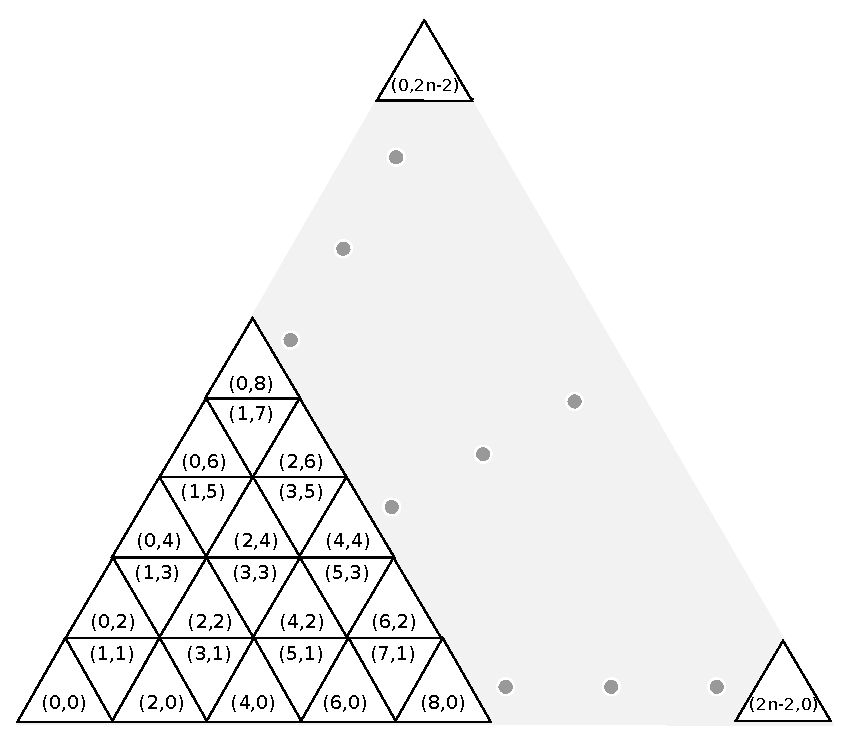
\includegraphics{./images/triTriGrid.eps}
 \caption{Grid generated by \texttt{triTriGrid}}
\end{figure}


\texttt{paraTriGrid r c} returns a grid in the shape of a parallelogram with
\texttt{r} rows and \texttt{c} columns, using triangular tiles.
The indexing scheme is illustrated in Figure \ref{fig:paraTriGrid}.

\begin{figure}[ht]
 \label{fig:paraTriGrid}
 \centering
 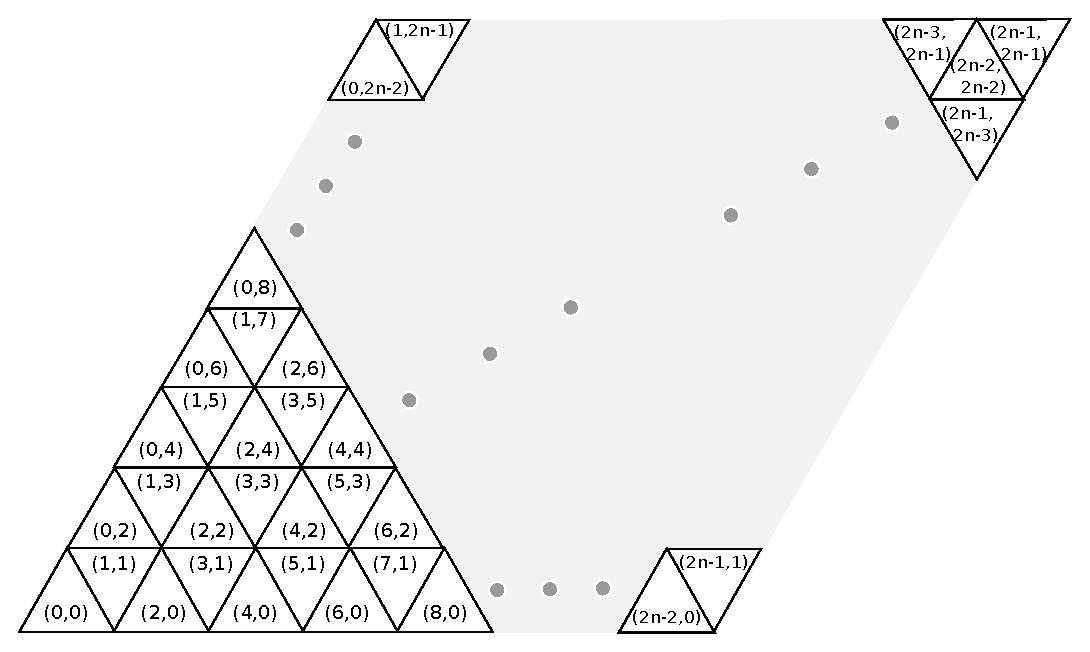
\includegraphics[scale=0.9,keepaspectratio=true]{./images/paraTriGrid.eps}
 \caption{Grid generated by \texttt{paraTriGrid}}
\end{figure}


\section{Hexagonal tiles}

\texttt{hexHexGrid s} returns a grid of hexagonal shape, with
sides of length \texttt{s}, using hexagonal tiles. 
The indexing scheme is illustrated in Figure \ref{fig:hexHexGrid}.

\begin{figure}[ht]
 \label{fig:hexHexGrid}
 \centering
 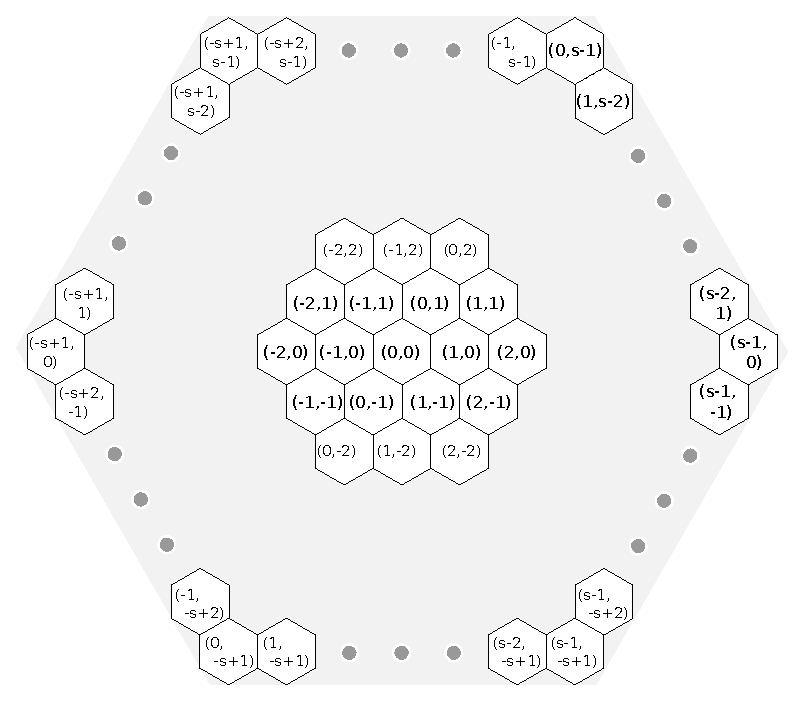
\includegraphics{./images/hexHexGrid.eps}
 \caption{Grid generated by \texttt{hexHexGrid}}
\end{figure}


\texttt{paraHexGrid r c} returns a grid in the shape of a parallelogram with \texttt{r} rows and \texttt{c} columns, using hexagonal tiles. 
The indexing scheme is illustrated in Figure \ref{fig:paraHexGrid}.

\begin{figure}[ht]
 \label{fig:paraHexGrid}
 \centering
 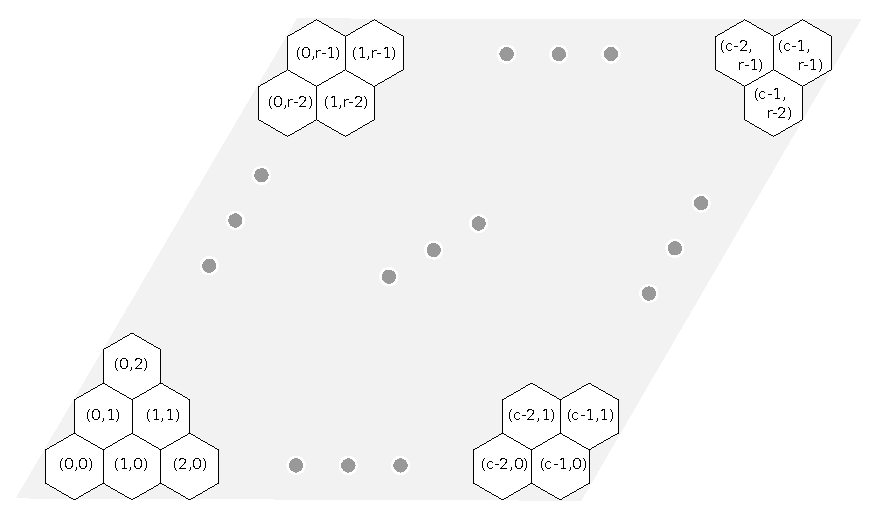
\includegraphics{./images/paraHexGrid.eps}
 \caption{Grid generated by \texttt{paraHexGrid}}
\end{figure}

\end{document}
